% 평가문항 만들어 봅시다.
\documentclass[a4paper,11pt,fleqn]{article}   % 2단 편집에서 ,twocolumn 있었어.

\usepackage{kotex}
\usepackage{amssymb}
\usepackage{gensymb}
\usepackage{color}
\usepackage{array}
\usepackage{graphicx}
\DeclareGraphicsExtensions{.pdf,.png,.jpg}

\usepackage{amsmath}
\usepackage{hyperref}

\usepackage[left=1.5cm,right=1.5cm,top=2.5cm,bottom=3cm,a4paper]{geometry}      % 여백을 조정
\usepackage[onehalfspacing]{setspace}   % 줄간격 옵션 singlespacing, onehalfspacing, doublespacing

% \setlength{\columnseprule}{0.5pt}    % 2단 편집에서 가운데 줄 

\usepackage{fancyhdr}
\usepackage{lastpage}

\pagestyle{fancy}
\lhead{} 
\chead{\Large{\sf{\textbf{2023학년도 3학년 (해석역학 입문) (1)학기 (2)차 지필평가 문항지} }}}			%%% 과목, 학기, 차
\rhead{}
\lfoot{\rule{\linewidth}{0.7pt}} 
\cfoot{$ $ \n    \thepage \hspace{1pt} / \hspace{1pt} \pageref{LastPage} } 
\rfoot{$ $ \n    \sf{\textbf{과학영재학교 광주과학고등학교}}}

\usepackage{verbatim}
\usepackage{enumitem}

\newcommand{\n}{\newline}


	



\begin{document}


\begin{tabular}{m{.13\linewidth}
		m{.30\linewidth}} 
	\large{평가실시일 :}& \large{2023년 (6)월 (27)일 (3-4)교시} \\										%%% 고사실시일 
	\large{문 \hspace{3pt} 항 \hspace{3pt} 수 :} & \large{총 (6)문항} \\	   		   	       			    %%% 문항수
	\large{} & \large{단답형 ()개, 서술형 ()개} \\
\end{tabular}
\begin{tabular}{|
		>{\centering}m{.12\linewidth}|
		>{\centering}m{.10\linewidth}|
		>{\centering}m{.10\linewidth}|
		>{\centering}m{.10\linewidth}|} \hline
	출제교사&부장&교감&교장 \tabularnewline \hline
	최용석 \hspace{1pt} (인)&{}&{}&{} \tabularnewline
	정현주 \hspace{1pt} (인)&{}&{}&{} \tabularnewline
	{}&{}&{}&{} \tabularnewline
	\hline
\end{tabular}
\n


\rule{\linewidth}{0.5pt} \n


\begin{tabular}{|m{.96\linewidth}|} \hline
	\sffamily{
		[유의사항] \n
		⑴ 단답형, 서술형 답안은 검은색 또는 파란색 볼펜을 사용하여 작성합니다. \n
		⑵ 서술형 문항은 풀이 과정 없이 답만 있는 경우 0점 처리됩니다. \n
		⑶ 답안은 정돈된 글씨로 작성하며, 알아볼 수 없는 글씨는 감점할 수 있습니다.}
	\\ \hline
\end{tabular}
\n\n\n
-1- 내가 단답 6점, 서술 29점 내면 되는가? 
\newpage
-2-
\newpage
-3-
\newpage
-4-
\newpage



\begin{center}
	$\blacksquare \blacksquare \blacksquare$ \textbf{단답형} $\blacksquare \blacksquare \blacksquare$
\end{center}

\begin{enumerate}[start=12]
	
	%%%%%%%%%%%%%%%%%%%%%%%%%%%%%%%%%%%%%%%%%%%%%%%%%%%%% 단답형 12번
	\item 변의 길이가 $a$, $b$인 균일한 직사각형 판의 중심에서의 주관성모멘트(principal moments of inertia)를 구하시오.  [6점]
	\begin{figure}[h]
		\begin{center}
			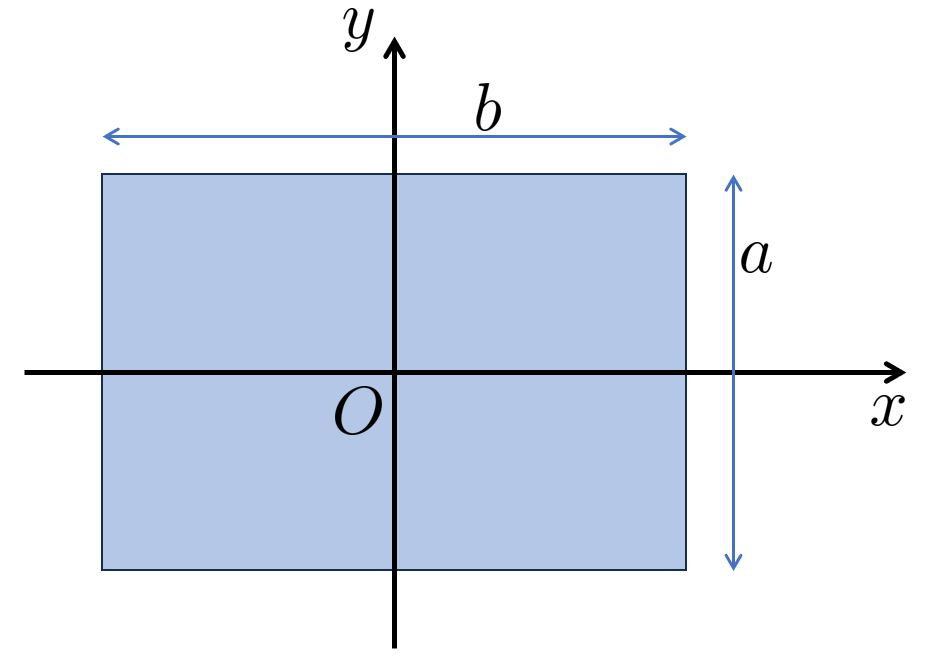
\includegraphics[scale=0.3]{img/rectangle}
			%\caption{캡션} \label{fig:label}
		\end{center}
	\end{figure}
\n\n\n
	
\end{enumerate}

\begin{center}
$\blacksquare \blacksquare \blacksquare$ \textbf{서술형} $\blacksquare \blacksquare \blacksquare$
\end{center}

\begin{enumerate}[start=13]

	%%%%%%%%%%%%%%%%%%%%%%%%%%%%%%%%%%%%%%%%%%%%%%%   서술형 13번
	\item 질량이 $2$, $1$, $4$인 입자들이 각각 $(1, -1, 1)$, $(2, 0, 2)$, $(-1,1,0)$에 고정되어 있는 강체가 있다. 이들이 각속도 $\vec{\omega} = 3 \hat{i} -2 \hat{j} +4 \hat{k}$로 회전한다면 각운동량은 얼마인가?  [7점]
\n\n\n\n\n\n\n\n

	%%%%%%%%%%%%%%%%%%%%%%%%%%%%%%%%%%%%%%%%%%%%%%%%%%%%%%%%%%%%%%%%%%%%%%%%%%%%%%%%%%%%%%%%%%% 14번. 10.43
	\item 위 13번의 강체에 대하여 $x$, $y$, $z$ 각 축에 대한 관성모멘트 및 관성곱들을 계산하여 관성모멘트 텐서를 구하시오. [6점]	
\n
\[
	\tilde{I} = \begin{pmatrix}
		I_{xx} & I_{xy} & I_{xz} \\
		I_{yx} & I_{yy} & I_{yz} \\
		I_{zx} & I_{zy} & I_{zz}
	\end{pmatrix} = \cdots
\]
\n\n
	
	
	
\newpage		
	
	%%%%%%%%%%%%%%%%%%%%%%%%%%%%%%%%%%%%%%%%%%%%%%%%%%%%%%%%%%%%%%%%%%%%%%%%%%%%%%%%%%%%%%%%%  15번. 10.46
	\item 한 변의 길이가 $a$인 정육면체 강체의 모서리가 $x$축, $y$축, $z$축과 일치해 있다. [6점] \n
	원점에 대하여 \n
	
	\begin{figure}[h]
		\begin{center}
			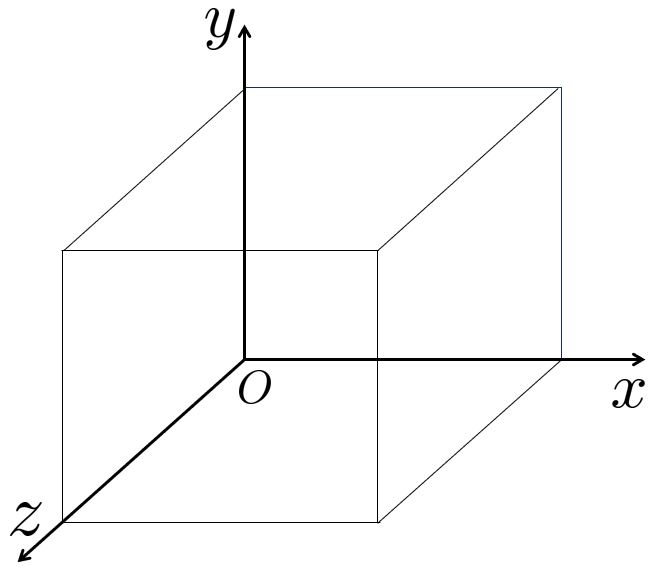
\includegraphics[scale=0.4]{img/cube}
			%\caption{캡션} \label{fig:label}
		\end{center}
	\end{figure}	
	
	(a) 각 축에 대한 관성모멘트를 구하시오. \n\n
	(b) 각 관성곱들을 구하시오. 
\n\n\n

	%%%%%%%%%%%%%%%%%%%%%%%%%%%%%%%%%%%%%%%%%%%%%%%%%%%%%%%%%%%%%%%%%%%%%%%%%%%%%%%%%%%%%%%%%%%% 16번.  10.47
	\item 위 15번의 강체가 $O$에 대하여 $\vec{\omega}= 2\hat{i}+5\hat{j}-3\hat{k}$의 각속도로 회전하고 있다.  [6점]\n
	(a) 원점 $O$에 대한 각운동량을 구하시오. \n\n
	(b) 원점 $O$에 대한 회전운동에너지를 구하시오.
\n\n\n
	
	
	%%%%%%%%%%%%%%%%%%%%%%%%%%%%%%%%%%%%%%%%%%%%%%%%%%%%%%%%%%%%%%%%%%%%%%%%%%%%%%%%  17번. 10.49
	\item 질량이 각각 $m_1$, $m_2$인 두 개의 입자가 질량을 무시할 수 있는 막대(길이는 $l$)로 연결돼 있다. 이 강체의 주관성모멘트를 찾으시오.(좌표계의 원점 $O$는 질량중심에 잡고, 그림을 그려 설명하시오.) [4점]
	\n

\end{enumerate}
.
\\[1.5cm]
%\rule{.96\linewidth}{0.8pt}
%\centering{ 수고하셨습니다. }\n
\begin{center}
	$\blacksquare \blacksquare \blacksquare$ \textbf{수고하셨습니다.} $\blacksquare \blacksquare \blacksquare$
\end{center}


\begin{tabular}{|m{.9\linewidth}|} \hline
\sffamily{이 시험 문제의 저작권은 광주과학고등학교에 있습니다. 저작권법에 의해 보호받는 저작물이므로 전재와 
	복제는 금지되며, 이를 어길 시 저작권법에 의거 처벌될 수 있습니다.}
\\ \hline
\end{tabular}

 

\begin{comment}
	
\begin{displaymath}
	
\end{displaymath}

\begin{eqnarray*}
	e^{2i \theta} &=& cos 2 \theta + i sin 2 \theta \\
	( e^{i \theta} ) ^2  &=& ( cos \theta + i sin \theta ) ^2 = cos ^2 \theta - sin ^2 \theta + 2 i cos \theta sin \theta
\end{eqnarray*}

\begin{equation}
	%sin 3 \theta = 3sin \theta - 4 sin ^3 \theta
\end{equation}

%\begin{figure}[htbp] 옵션 here, top, bottom, page of floats
\begin{figure}[h]
	\begin{center}
	    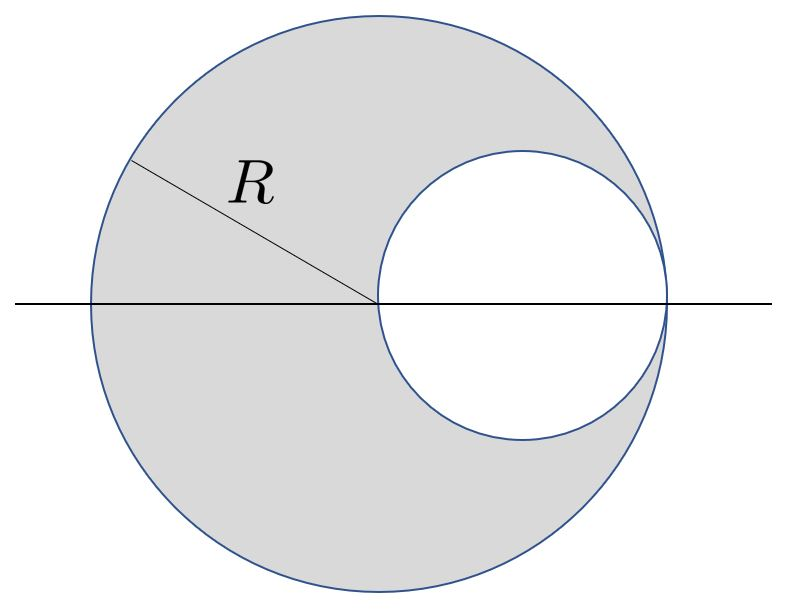
\includegraphics[scale=0.9]{img/17q}
	    %\caption{캡션} \label{fig:label}
	\end{center}
\end{figure}
	
\textcolor{blue}{색깔 있는 글자}

\rule{\linewidth}{1pt}  긴 줄을 긋고 

\newline  새 줄로


% watermark text 
%%%%%%%%%%%%%%%%%%%%%%%%%%%%%%%%%%%%%%%
\usepackage[printwatermark]{xwatermark}
\usepackage{xcolor}
%\usepackage{lipsum}
\newwatermark[allpages,color=blue!30,angle=60,scale=3,xpos=0,ypos=0]{ds4dqs@gsa.hs.kr}
%%%%%%%%%%%%%%%%%%%%%%%%%%%%%%%%%%%%%%


% watermark picture
%%%%%%%%%%%%%%%%%%%%%%%%%%%%%%%%%%%%%%%
\usepackage{background}
\backgroundsetup{scale=0.4, angle=0, firstpage=true, opacity=0.2, contents=\includegraphics{image/gsa2.png}}
%%%%%%%%%%%%%%%%%%%%%%%%%%%%%%%%%%%%%%



\end{comment}

\end{document}
